\documentclass[11pt]{article}
\usepackage[margin=1in]{geometry}
\usepackage{amsmath,amssymb,amsthm}
\usepackage{graphicx}
\usepackage[colorlinks=true,linkcolor=blue,citecolor=blue,urlcolor=blue]{hyperref}
\newtheorem{theorem}{Theorem}[section]
\newtheorem{lemma}[theorem]{Lemma}
\newtheorem{proposition}[theorem]{Proposition}
\newtheorem{corollary}[theorem]{Corollary}
\newtheorem{definition}[theorem]{Definition}
\theoremstyle{remark}
\newtheorem{remark}[theorem]{Remark}
\newcommand{\Tr}{\operatorname{Tr}}
\newcommand{\kms}[1]{\|#1\|_{2,\sigma}}

\title{Finite-Dimensional Davies Interface Lemmas and TFIM Witness Tests\\
for Separation-Dependent Decoherence Rate Envelopes\\
{\normalsize Version 2}}
\author{Lluis Eriksson\\ Independent Researcher\\ \texttt{lluiseriksson@gmail.com}}
\date{January 2026 (v1); July 2026 (v2)}

\begin{document}
\maketitle

\begin{abstract}
We develop a finite-dimensional technical core for relating separation to
effective decoherence-rate envelopes in Davies-type open-system dynamics.
We work with energy pinching $\Delta$ and quantify coherence by
$C(\rho) = S(\rho\|\Delta[\rho])$. We import a maintenance inequality
$P_{\rm extra}(\rho) \ge k_B T\, \dot C_{\rm loss}(\rho)$ -- in the
corrected operational sense of its source (paired strategies against
efficient/free baselines, 2512.0061 v2) -- as an external input. On the operator side we prove: (i) an exact $\omega = 0$ Dirichlet
identity yielding a witness-based lower bound on instantaneous decay
envelopes, (ii) a Bohr-channel Dirichlet decomposition for a single-channel
Davies generator under quantum detailed balance -- \emph{corrected in v2}:
the v1 form $\frac12\sum_\omega \gamma(\omega)\|[S(\omega),O]\|^2_{2,\sigma}$
is false as an identity (numerical deviations of order $20\%$); the exact
form is $\sum_\omega \gamma(\omega) e^{\beta\omega/2}\,
\Re\langle S(\omega)O, [S(\omega),O]\rangle_\sigma$, which reduces to (i) at
$\omega = 0$ and is nonnegative pairwise in $\pm\omega$ -- and (iii)
envelope suppression lemmata under infrared exclusion and quasi-local
spectral tails, \emph{reproved in v2}: the v1 proofs used a KMS
submultiplicativity step that is false in general (a one-qubit
counterexample saturates the corrected constant); the corrected constants
carry $c_\sigma^2 = (\lambda_{\max}/\lambda_{\min})^{1/2}$ and
$\sup_\omega \gamma(\omega)e^{\beta\omega/2}$, and the $e^{-2\epsilon/\xi}$
exponent survives via a new \emph{positivity-pinning} argument: for
$S = S_{\rm near} + \delta\, S_{\rm tail}$ and far-supported $O$, detailed
balance at every $\delta$ forces $\mathcal{E}_\delta(O) = \delta^2
\mathcal{E}_{\rm tail}(O)$ exactly. Consequently Lemma 4.13's v1 claim of a
$\lambda_{\min}(\sigma)$-free prefactor is downgraded to a quadratically
improved dependence. On the state side we give an asymptotic linearization
on Bohr-block perturbations with fixed diagonal, yielding a
direction-dependent effective decay rate. Finite-size TFIM witness
diagnostics are provided, and every corrected statement is verified to
machine precision by the shipped suite.
\end{abstract}

\paragraph{Summary of results and assumptions (updated in v2).}
Imported: the maintenance inequality (Theorem~\ref{thm:maint}) from
\cite{S0061}. Proved here (finite dimension): Lemma~\ref{lem:omega0},
Lemma~\ref{lem:mult} (new), Lemma~\ref{lem:bohr} (corrected),
Lemma~\ref{lem:pin} (new), Proposition~\ref{prop:witness},
Lemmas~\ref{lem:sup1}--\ref{lem:sup2} (corrected constants),
Proposition~\ref{prop:lin} and Corollary~\ref{cor:eig}. Finite-size
numerics: Section~\ref{sec:tfim}. No thermodynamic-limit claims. All
identities and counterexamples are verified in
\texttt{verification/2601-0023/} (Section~\ref{sec:verif}).

\section{Scope, positioning, and non-claims}
This manuscript is finite-dimensional and makes no thermodynamic-limit
claims unless stated. It does not propose modified dynamics, collapse
mechanisms, Born-rule derivations, or ontological resolutions of the
measurement problem. For theorem-level frameworks relating correlation
decay and log-Sobolev inequalities see \cite{Capel, CM}; our aim is an
operator/state interface around Davies Dirichlet forms and a witness
floor, with reproducible finite-size diagnostics. \emph{Series context
(added in v2):} this note is the theory core behind the TFIM witness
diagnostics of 2601.0022 \cite{S0022} (whose ED parameters are the ones
declared in Appendix~A here), and feeds the $\omega = 0$-floor block
2512.0064/2512.0070 \cite{S0064, S0070} and the entropic interface
2601.0020 \cite{S0020}.

\section{Finite-dimensional operational core}
Let $H_S = \sum_n E_n \Pi_n$, $\sigma := e^{-\beta H_S}/\Tr(e^{-\beta H_S})$,
$\Delta[\rho] := \sum_n \Pi_n \rho \Pi_n$, and
$C(\rho) := S(\rho\|\Delta[\rho])$ with Umegaki relative entropy. If $H_S$
is degenerate, $\Delta$ is energy-\emph{block} pinching and $S(0)$ below is
block-diagonal on degenerate subspaces (the numerics group energies within
$10^{-10}$). The uncontrolled evolution is a GKLS semigroup with
$\mathcal{L}(\sigma) = 0$; $\dot C_{\rm loss}(\rho) := -\frac{d}{dt}
C(\rho_t)|_{t=0}$. Battery-assisted thermal operations define
$P_{\rm extra}(\rho) := \inf\,[P(s) - P(s_{\rm diag})]$ over paired
strategies maintaining $\rho$ resp.\ $\Delta[\rho]$.
\begin{theorem}[Imported maintenance inequality \cite{S0061}]
\label{thm:maint}
If ${\rm Ctrl}(\rho) \neq \emptyset$ and ${\rm Ctrl}(\Delta[\rho]) \neq
\emptyset$, then $P_{\rm extra}(\rho) \ge k_B T\, \dot C_{\rm loss}(\rho)$,
with $P_{\rm extra}$ understood in the corrected operational sense of
2512.0061 v2 (paired strategies against efficient/free baselines; the v1
``assumption-free'' variant of that source was vacuous and is not used
here).
\end{theorem}

\section{Davies generators, KMS Dirichlet form, and a separation envelope}
Fix $S = S^\dagger$ and a Davies generator in the weak-coupling--secular
limit, with Bohr components $S(\omega) := \sum_{E_m - E_n = \omega} \Pi_m S
\Pi_n$, $S(\omega)^\dagger = S(-\omega)$, and KMS rates $\gamma(-\omega) =
e^{-\beta\omega}\gamma(\omega)$. Define $\langle A, B\rangle_\sigma :=
\Tr(\sigma^{1/2}A^\dagger \sigma^{1/2} B)$,
$\mathcal{E}_\sigma(O) := -\Re\langle O, \mathcal{L}^\dagger(O)
\rangle_\sigma$, far regions $\Omega_\epsilon := \{j : d(j, \Omega_0) \ge
\epsilon\}$ with observable subspace $\mathcal{A}_\epsilon$, and
$\kappa(\epsilon) := \sup_{O \in \mathcal{A}_\epsilon}
\mathcal{E}_\sigma(O)/\kms{O}^2$.
\begin{remark}[Modular relations]
\label{rem:modular}
Since $(S(\omega))_{mn} \neq 0$ only if $E_m - E_n = \omega$:
$\sigma^s S(\omega) \sigma^{-s} = e^{-s\beta\omega} S(\omega)$ for all $s$,
and $S(\omega)^\dagger S(\omega)$ commutes with $\sigma$. These two facts
drive all corrected identities below.
\end{remark}

\section{Interface lemmas}
\subsection{The $\omega = 0$ channel yields a witness floor}
\begin{lemma}[Exact $\omega = 0$ Dirichlet identity]
\label{lem:omega0}
Assume $[S(0), H_S] = 0$ and $\gamma(0) > 0$. For the $\omega = 0$ Davies
channel $\mathcal{L}_0^\dagger(O) = \gamma(0)(S(0)OS(0) -
\tfrac12\{S(0)^2, O\})$, one has $\mathcal{E}^{(0)}_\sigma(O) =
\tfrac{\gamma(0)}{2}\, \kms{[S(0), O]}^2$ for all $O$.
\end{lemma}
\begin{proof}
As in v1: with $L := S(0)$, $[L, \sigma^{1/2}] = 0$ makes left/right
multiplication by $L$ KMS-self-adjoint; expanding
$\langle[L,O],[L,O]\rangle_\sigma$ gives the identity. (Verified to
$4\times10^{-16}$ in the suite.)
\end{proof}

\subsection{Bohr-channel Dirichlet decomposition (corrected in v2)}
\begin{remark}[The v1 decomposition is false as an identity]
\label{rem:43false}
v1 asserted $\mathcal{E}_\sigma(O) = \frac12 \sum_\omega \gamma(\omega)
\kms{[S(\omega), O]}^2$, citing the divergence-form representation of
\cite{CM}. That representation involves \emph{modular-deformed}
derivations, not plain commutators; the plain-commutator form is exact only
at $\omega = 0$. On a TFIM $N = 4$ single-channel Davies model the suite
finds relative deviations up to $0.22$ between $\mathcal{E}_\sigma$ and the
v1 right-hand side.
\end{remark}
\begin{lemma}[Bohr-channel Dirichlet decomposition, corrected]
\label{lem:bohr}
Under quantum detailed balance and the single-channel Davies form,
for Hermitian $O$,
\[
\mathcal{E}_\sigma(O) \;=\; \sum_\omega \gamma(\omega)\, e^{\beta\omega/2}\,
\Re\,\bigl\langle S(\omega) O,\; [S(\omega), O] \bigr\rangle_\sigma .
\]
Each pair $\{+\omega, -\omega\}$ of summands is jointly nonnegative
(each such pair, with its KMS rates, is itself a detailed-balanced
generator), and the $\omega = 0$ summand equals
$\mathcal{E}^{(0)}_\sigma(O)$ of Lemma~\ref{lem:omega0}.
\end{lemma}
\begin{proof}
Per channel, using Remark~\ref{rem:modular}:
$\langle O, S(\omega)^\dagger O S(\omega)\rangle_\sigma =
e^{\beta\omega/2}\langle S(\omega) O, O S(\omega)\rangle_\sigma$ and
$\langle O, S(\omega)^\dagger S(\omega) O\rangle_\sigma =
\Re\,\langle O, O S(\omega)^\dagger S(\omega)\rangle_\sigma =
e^{\beta\omega/2}\kms{S(\omega) O}^2$ (move $\sigma^{1/2}$ through
$S(\omega)^\dagger$, use $[S^\dagger S, \sigma] = 0$ and cyclicity).
Substituting into $-\Re\langle O, \mathcal{L}^\dagger_\omega(O)
\rangle_\sigma$ gives the $\omega$ summand
$\gamma(\omega)e^{\beta\omega/2}[\kms{S(\omega)O}^2 -
\Re\langle S(\omega)O, OS(\omega)\rangle_\sigma]$. Pairwise nonnegativity
follows since the $\{\pm\omega\}$ sub-generator is KMS-symmetric with
stationary $\sigma$, hence has nonnegative Dirichlet form. At $\omega = 0$,
$\kms{OS(0)} = \kms{S(0)O}$ (adjoint invariance of the KMS norm), and the
summand equals $\tfrac{\gamma(0)}{2}\kms{[S(0),O]}^2$. All statements are
verified to machine precision in the suite ($2\times10^{-16}$).
\end{proof}

\subsection{Witness floor}
\begin{proposition}[Witness lower bound at fixed separation]
\label{prop:witness}
In the setting of Lemma~\ref{lem:bohr}, fix $\epsilon_0 \ge 1$. If there is
$O_{\epsilon_0} \in \mathcal{A}_{\epsilon_0}$ with
$\kms{[S(0), O_{\epsilon_0}]}^2 / \kms{O_{\epsilon_0}}^2 \ge c_{\epsilon_0}
> 0$, then $\kappa(\epsilon_0) \ge \tfrac{\gamma(0)}{2} c_{\epsilon_0}$.
\end{proposition}
\begin{proof}
By Lemma~\ref{lem:bohr}, $\mathcal{E}_\sigma \ge$ its $\omega = 0$ summand
(the remaining $\pm\omega$ pairs are jointly nonnegative), which equals
$\mathcal{E}^{(0)}_\sigma$; apply Lemma~\ref{lem:omega0}. (Note the v1
proof used termwise nonnegativity of the -- incorrect -- commutator
decomposition; pairwise nonnegativity suffices.)
\end{proof}

\subsection{KMS multiplication bound (new in v2)}
\begin{lemma}[KMS multiplication bound and sharpness]
\label{lem:mult}
For all $X, O$: $\kms{XO} \le \|\sigma^{1/4} X \sigma^{-1/4}\|_\infty
\kms{O} \le c_\sigma \|X\|_\infty \kms{O}$, and likewise for $OX$, with
$c_\sigma := (\lambda_{\max}(\sigma)/\lambda_{\min}(\sigma))^{1/4}$. The
naive bound $\kms{XO} \le \|X\|_\infty \kms{O}$, used implicitly in v1's
Lemmas 4.12--4.13, is false: for one qubit with gap $\Delta$,
$X = \sigma^x$ and $O = |1\rangle\langle 0|$ give $\kms{XO}/\kms{O} =
e^{\beta\Delta/4}$, which saturates $c_\sigma$.
\end{lemma}
\begin{proof}
$\kms{A} = \|\sigma^{1/4} A \sigma^{1/4}\|_2$, so $\kms{XO} =
\|(\sigma^{1/4}X\sigma^{-1/4})(\sigma^{1/4}O\sigma^{1/4})\|_2 \le
\|\sigma^{1/4}X\sigma^{-1/4}\|_\infty \kms{O}$, and
$\|\sigma^{1/4}X\sigma^{-1/4}\|_\infty \le \lambda_{\max}^{1/4}
\lambda_{\min}^{-1/4}\|X\|_\infty$. The one-qubit computation is direct.
(300 random draws in the suite: no violations of the corrected bound.)
\end{proof}

\subsection{Envelope suppression (reproved in v2)}
Definitions of IR exclusion at $\omega^* $, tensor lattice, support, tail
map $\mathrm{tail}_\epsilon(X) := X - E_{<\epsilon}(X)$, and the norm
comparison $\|X\|_2^2 \le \lambda_{\min}(\sigma)^{-1}\kms{X}^2$ are as in
v1 (that lemma is correct).
\begin{lemma}[Positivity pinning (new in v2)]
\label{lem:pin}
Let $O$ be supported on $\Omega_\epsilon$ and decompose each coupling as
$S = S_{\rm near} + S_{\rm tail}$ with $S_{\rm near} :=
E_{<\epsilon}(S)$. For $\delta \in \mathbb{R}$ let
$\mathcal{E}_\delta$ denote the Dirichlet form of the Davies generator
built from $S_{\rm near} + \delta S_{\rm tail}$ (same $H_S$, same rates).
Then
\[
\mathcal{E}_\delta(O) \;=\; \delta^2\, \mathcal{E}_{\rm tail}(O)
\qquad\text{exactly},
\]
where $\mathcal{E}_{\rm tail}$ is the Dirichlet form built from
$S_{\rm tail}$ alone.
\end{lemma}
\begin{proof}
Each $\delta$ yields a detailed-balanced Davies generator with stationary
$\sigma$, so $\delta \mapsto \mathcal{E}_\delta(O) \ge 0$ for all real
$\delta$. The dissipator is exactly quadratic in the coupling, so
$\mathcal{E}_\delta(O) = a + b\delta + c\delta^2$ with $a =
\mathcal{E}_{\rm near}(O) = 0$ (near jumps commute with far $O$) and $c =
\mathcal{E}_{\rm tail}(O)$. Nonnegativity of a quadratic vanishing at
$\delta = 0$ forces $b = 0$. (Verified exactly over four decades of
$\delta$ in the suite.)
\end{proof}
\begin{lemma}[Envelope suppression from KMS tails; corrected constant]
\label{lem:sup1}
Assume IR exclusion at $\omega^* > 0$ and
$\kms{\mathrm{tail}_\epsilon(S(\omega))} \le A(1+\epsilon)^p
e^{-\epsilon/\xi}$ for $|\omega| \ge \omega^*$, with
$\tilde\gamma_{\sup} := \sup_{|\omega|\ge\omega^*}
\gamma(\omega)e^{\beta\omega/2} < \infty$. Then for fixed $(N, \beta)$,
\[
\kappa(\epsilon) \le C (1+\epsilon)^{2p} e^{-2\epsilon/\xi},
\qquad
C := 2\, |\Omega_{\ge\omega^*}|\; \tilde\gamma_{\sup}\; c_\sigma^2\,
\lambda_{\min}(\sigma)^{-1} A^2 .
\]
\end{lemma}
\begin{lemma}[Envelope suppression from operator-norm tails; corrected]
\label{lem:sup2}
With the tail hypothesis in operator norm,
$\|\mathrm{tail}_\epsilon(S(\omega))\|_\infty \le A(1+\epsilon)^p
e^{-\epsilon/\xi}$, the same bound holds with
$C_\infty := 2\, |\Omega_{\ge\omega^*}|\; \tilde\gamma_{\sup}\;
c_\sigma^2\, A^2$.
\end{lemma}
\begin{proof}[Proof of Lemmas \ref{lem:sup1}--\ref{lem:sup2}]
By Lemma~\ref{lem:pin} (applied with $\delta = 1$),
$\mathcal{E}_\sigma(O) = \mathcal{E}_{\rm tail}(O)$ for far-supported $O$.
By Lemma~\ref{lem:bohr} applied to the tail generator and
Cauchy--Schwarz, each channel contributes at most
$\gamma(\omega)e^{\beta\omega/2}\, \kms{T(\omega)O}\,\kms{[T(\omega),O]}
\le 2 c_\sigma^2 \|T(\omega)\|_\infty^2 \kms{O}^2\,
\gamma(\omega)e^{\beta\omega/2}$ with $T(\omega) :=
\mathrm{tail}_\epsilon(S(\omega))$ (Lemma~\ref{lem:mult} twice). Sum over
$\Omega_{\ge\omega^*}$ and insert the tail hypothesis; for
Lemma~\ref{lem:sup1} convert $\|T\|_\infty \le \|T\|_2 \le
\lambda_{\min}^{-1/2}\kms{T}$.
\end{proof}
\begin{remark}[Corrected trade-off; v1's Remark 4.14 revised]
\label{rem:tradeoff}
v1 claimed Lemma~\ref{lem:sup2}'s prefactor is independent of
$\lambda_{\min}(\sigma)$. With the corrected multiplication bound this is
no longer true: $c_\sigma^2 = (\lambda_{\max}/\lambda_{\min})^{1/2} \le
\lambda_{\min}^{-1/2}$. The honest comparison is: KMS-tail version
$\sim \lambda_{\min}^{-3/2}$ (worst case), operator-tail version
$\sim \lambda_{\min}^{-1/2}$ -- a quadratic improvement, not
$\lambda_{\min}$-freeness. Both versions also replace
$\sup\gamma$ by $\sup\gamma(\omega)e^{\beta\omega/2}$, reflecting the
corrected decomposition. The $e^{-2\epsilon/\xi}$ \emph{exponent} of v1 is
confirmed: by Lemma~\ref{lem:pin} the cross (near$\times$tail) terms
vanish identically, which v1 had implicitly and incorrectly justified via
the plain-commutator decomposition.
\end{remark}

\section{TFIM witness diagnostics (finite size)}
\label{sec:tfim}
TFIM with open boundaries, $H_S = -J\sum \sigma^x_i \sigma^x_{i+1} -
h\sum \sigma^z_i$, $h > J$; coupling site $j_0 = \lfloor N/2 \rfloor$,
$S = \sigma^z_{j_0}$; witness ratio $R(\epsilon; O) := \kms{[S(0),
O]}^2/\kms{O}^2$ optimized over single-site Paulis at $k = j_0 \pm
\epsilon$. By Proposition~\ref{prop:witness}, $\kappa(\epsilon) \ge
\tfrac{\gamma(0)}{2} R_{\rm opt}(\epsilon)$ -- unaffected by the v2
corrections, since only the $\omega = 0$ channel enters.
\begin{figure}[h]\centering
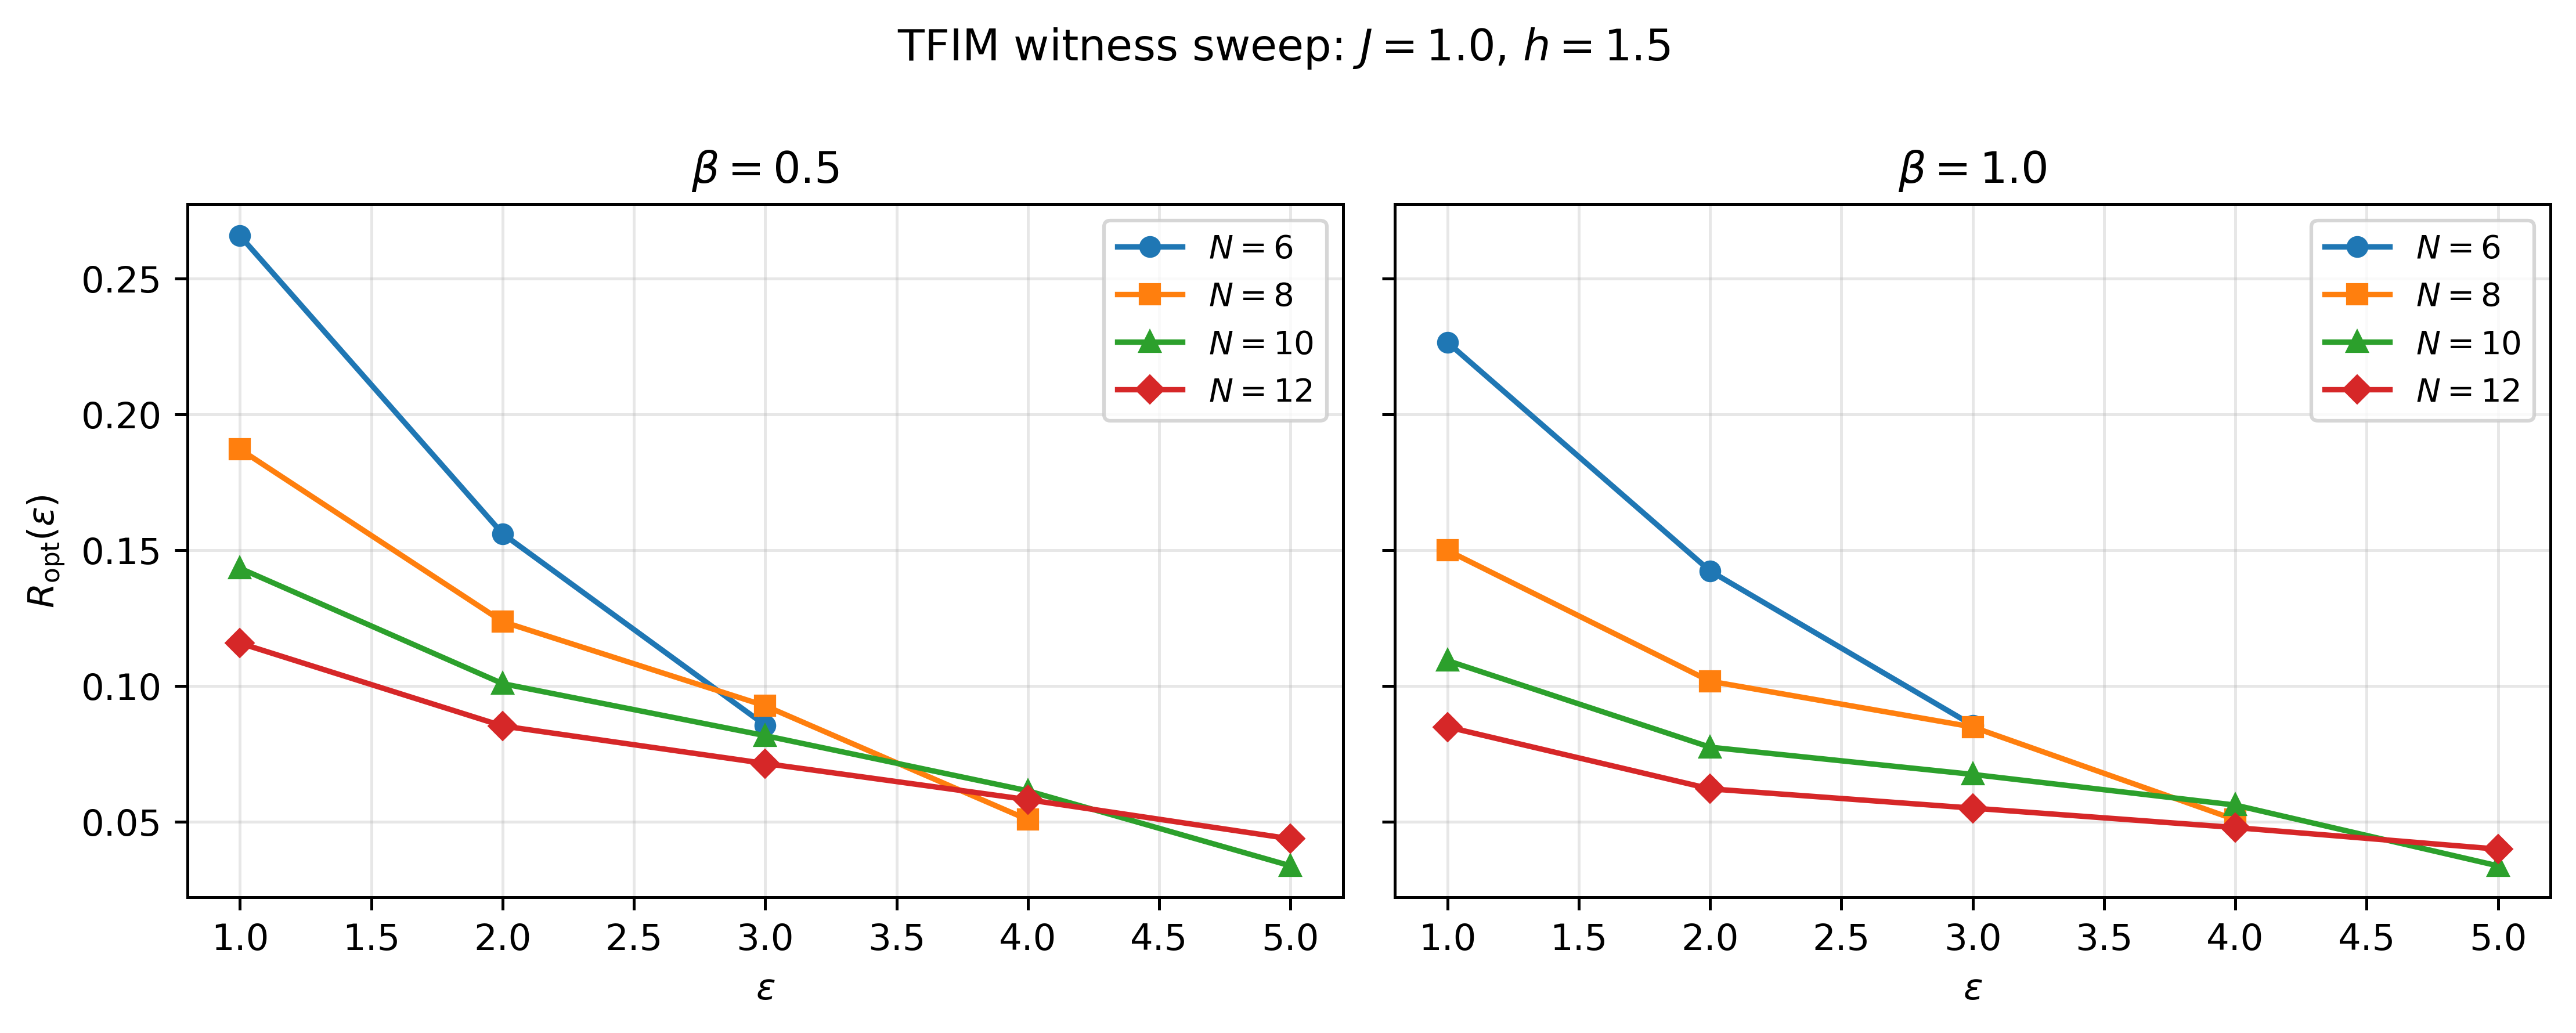
\includegraphics[width=0.95\textwidth]{fig1_ropt_sweep.png}
\caption{TFIM witness sweep at $J = 1.0$, $h = 1.5$: $R_{\rm opt}(\epsilon)$
for $N \in \{6, 8, 10, 12\}$, $\beta \in \{0.5, 1.0\}$. Exact
diagonalization with energy-block pinching.}
\end{figure}
\begin{figure}[h]\centering
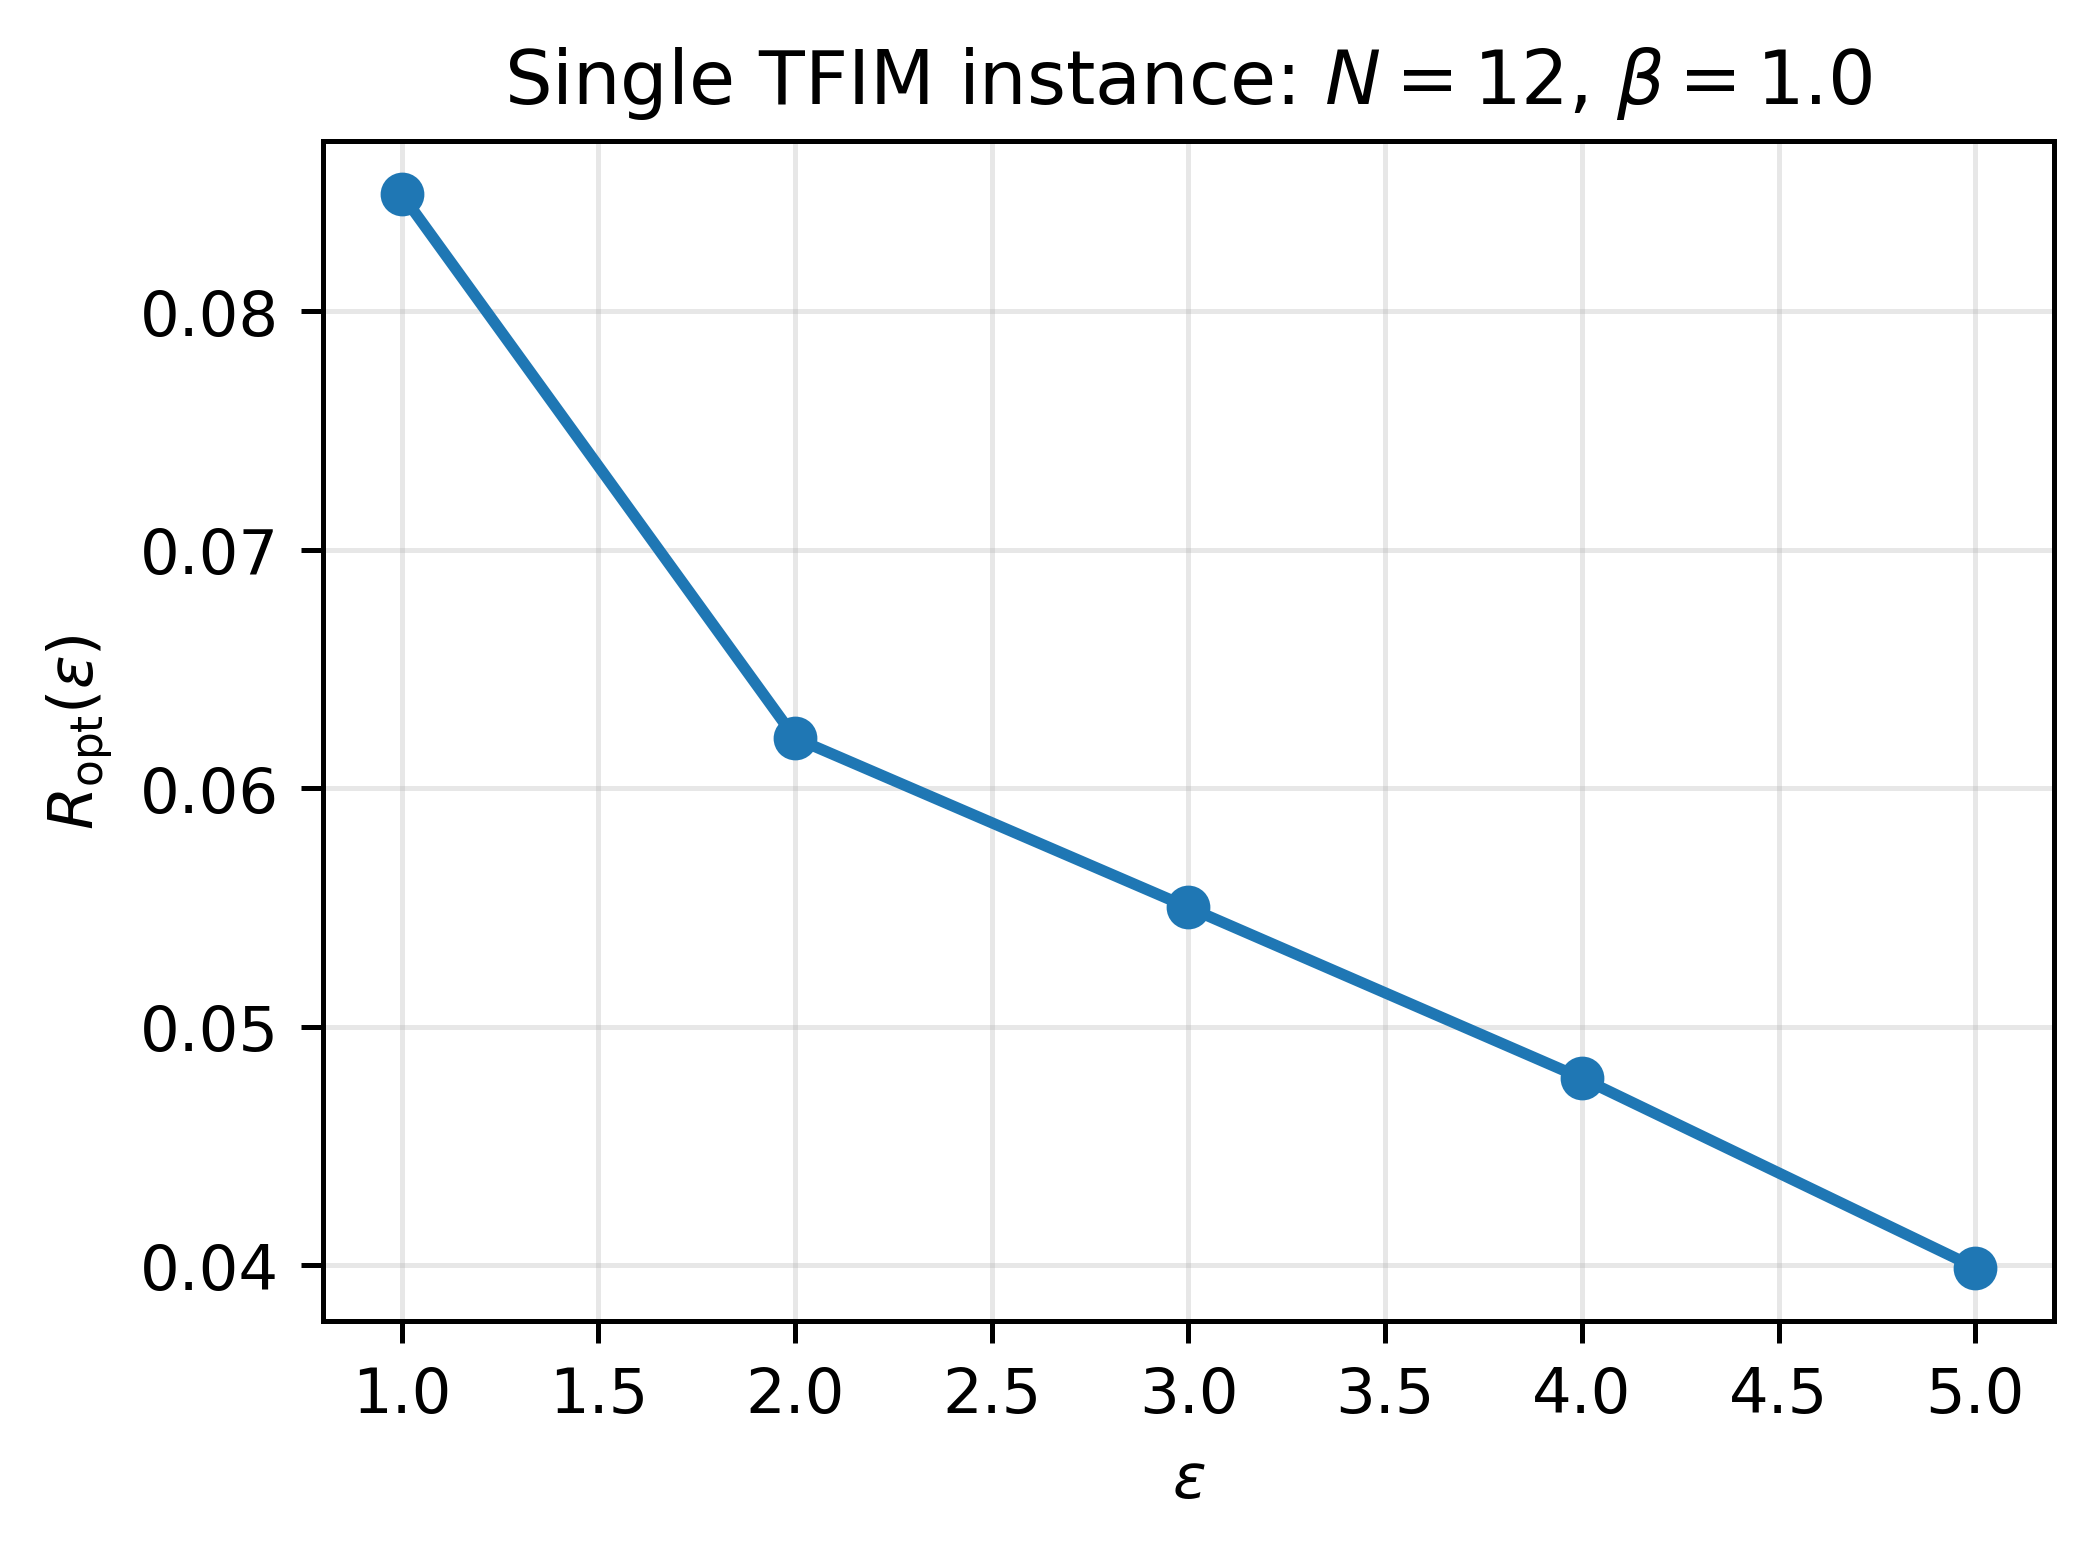
\includegraphics[width=0.55\textwidth]{fig2_ropt_single.png}
\caption{Single instance: $N = 12$, $\beta = 1.0$.}
\end{figure}

\section{State-side linearization (finite dimension)}
Definitions (BKM inner product, Bohr-block subspace $X_\Omega$) and the
quadratic expansion $S(\tau + \epsilon X\|\tau) = \tfrac{\epsilon^2}{2}
\langle X, X\rangle_{{\rm BKM},\tau} + O(\epsilon^3)$ are as in v1.
\begin{proposition}[Asymptotic interface on a Bohr block]
\label{prop:lin}
Let $\tau \succ 0$ be diagonal in the energy basis, $\mathcal{L}(\tau) =
0$, $\mathcal{L}(X_\Omega) \subseteq X_\Omega$, $X \in X_\Omega$ traceless,
$\rho(\epsilon) := \tau + \epsilon X$. Then $C(\rho(\epsilon)) =
\tfrac{\epsilon^2}{2}\langle X, X\rangle_{{\rm BKM},\tau} + O(\epsilon^3)$,
$\dot C_{\rm loss}(\rho(\epsilon)) = -\epsilon^2 \Re\langle X,
\mathcal{L}(X)\rangle_{{\rm BKM},\tau} + O(\epsilon^3)$, and
$\dot C_{\rm loss}/C = \Gamma_{\rm eff}(X) + O(\epsilon)$ with
$\Gamma_{\rm eff}(X) := -2\Re\langle X, \mathcal{L}(X)\rangle_{\rm BKM} /
\langle X, X\rangle_{\rm BKM}$.
\end{proposition}
\begin{corollary}[Eigenmode case]
\label{cor:eig}
If additionally $\mathcal{L}(X) = -\tfrac{\Gamma}{2}X$, then
$\Gamma_{\rm eff}(X) = \Gamma$ and $\dot C_{\rm loss} = \Gamma\,
C(\rho(\epsilon)) + O(\epsilon^3)$.
\end{corollary}

\section{Verification suite (added in v2)}
\label{sec:verif}
\texttt{verification/2601-0023/verify\_2601\_0023.py} verifies:
Lemma~\ref{lem:omega0} and the corrected Lemma~\ref{lem:bohr} to
machine precision on a TFIM $N = 4$ Davies model; the falsity of the v1
decomposition (deviations up to $0.22$); pairwise $\pm\omega$ positivity
(0 violations); the one-qubit counterexample of Lemma~\ref{lem:mult}
(ratio $= e^{\beta\Delta/4}$ exactly) and the corrected bound (0/300
violations); and the pinning identity of Lemma~\ref{lem:pin} exactly over
four decades of $\delta$. An optional flag \texttt{--with-tfim} runs the
$N = 10$ witness at the declared parameters ($J = 1$, $h = 1.5$,
$S = \sigma^z_{j_0}$), for comparison with the companion 2601.0022
\cite{S0022}, whose v1 ED used these parameters.

\section*{Note added in v2}
Three corrections, all verified in the suite; the witness mechanism and
all $\omega = 0$ statements of v1 stand unchanged.
(1) \emph{Lemma 4.3 (Bohr decomposition):} the v1 plain-commutator
identity is false in general (deviations $\sim 20\%$); the exact form is
Lemma~\ref{lem:bohr}, which reduces to the $\omega = 0$ identity and is
pairwise nonnegative -- the witness bound (Proposition~\ref{prop:witness})
survives with a repaired proof.
(2) \emph{Lemmas 4.12--4.13 (suppression):} the v1 proofs used the false
KMS submultiplicativity $\kms{XO} \le \|X\|_\infty\kms{O}$
(Lemma~\ref{lem:mult} gives the counterexample and the corrected
$c_\sigma$ bound); the corrected constants carry $c_\sigma^2$ and
$\sup\gamma(\omega)e^{\beta\omega/2}$, and v1's ``no
$\lambda_{\min}^{-1}$'' claim is downgraded per
Remark~\ref{rem:tradeoff}. The $e^{-2\epsilon/\xi}$ exponent is confirmed
by the new positivity-pinning Lemma~\ref{lem:pin}, which replaces the
incorrect route through the v1 decomposition.
(3) Series cross-references added; the appendix script is relocated to
\texttt{verification/2601-0023/} in the series repository (the inline
listing of v1 is superseded).

\appendix
\section{Reproducibility}
The TFIM figures were generated with
\texttt{tfim\_witness\_ropt\_all.py --J 1.0 --h 1.5 --eps\_max 5
--sweep\_N 6 8 10 12 --sweep\_beta 0.5 1.0 --single\_N 12
--single\_beta 1.0}. In v2 the script and the full verification suite
live in \texttt{verification/2601-0023/} of the series repository; the
inline listing of v1 is superseded.

\begin{thebibliography}{12}
\bibitem{S0061} L. Eriksson, \emph{The Conditional Maintenance Work
Theorem}, ai.viXra:2512.0061 (2025; v2 2026).
\bibitem{Davies} E. B. Davies, Commun. Math. Phys. \textbf{39} (1974)
91--110.
\bibitem{BP} H.-P. Breuer and F. Petruccione, \emph{The Theory of Open
Quantum Systems}, Oxford University Press (2002).
\bibitem{Capel} A. Capel, C. Rouz\'e, D. Stilck Fran\c{c}a,
arXiv:2009.11817.
\bibitem{CM} E. A. Carlen and J. Maas, J. Stat. Phys. \textbf{178} (2020)
319--378.
\bibitem{S0022} L. Eriksson, ai.viXra:2601.0022 (2026; v2 2026).
\bibitem{S0064} L. Eriksson, ai.viXra:2512.0064 (2025; v2 2026).
\bibitem{S0070} L. Eriksson, ai.viXra:2512.0070 (2025; v2 2026).
\bibitem{S0020} L. Eriksson, ai.viXra:2601.0020 (2026; v2 2026).
\end{thebibliography}
\end{document}
